\chapter{Approach I- Open edX intregation}
After testing our hybrid local intregation, and setting up our developing environment for Open edX,
the next phase was to integrate it with the running instance of Open edX on our Devstack
\section{Plan of action}
The idea and plan behind intregating our running hybrid instance of CodeMirror in TinyMCE with
Open edX is mentioned below:
\begin{enumerate}
\item\textbf{Indentation and code folding features}
\begin{itemize}
\item Add the latest version of CodeMirror v5.38.0 to the source code of Open edX
leaving the older version untouched.
\item Configure TinyMCE to open the updated version of CodeMirror as its raw HTML
editor.
\item Test the updated CodeMirror in TinyMCE and see if its wroking as expected.
\end{itemize}
\item\textbf{Enabling internal CSS}
\begin{itemize}
\item Understand the working of the XModule html\_module.py which is the widget
which loads the WYSIWYG editor in Open edX.
\item Learn how the html content is getting stored in the MongoDB .
\item The idea was to wrap the html content inside an inframe before it gets stored in the
Database. However this was to be done only when the course authors used internal
CSS in thier courses.
\item Similarly, while loading the content in LMS, it would be wrapped inside and iframe
first and then rendered in order to produce the desired effect.
\end{itemize}
\end{enumerate}

\section{Implementation}
\subsection{Configuring TinyMCE to use updated CodeMirror v5.38.0}
\begin{itemize}
\item The CodeMirror and TinyMCE source files are located in the edx-platfrom can be found on
the following path : \textit{\textbf{edx-platform/common/statis/js/vendor}}
\item Inside the tinymce source code, we placed the updated version of CodeMirror in the plugins
folder for TinyMCE.\newline The path was :
\textit{\textbf{edx-platform/common/static/js/vendor/tinymce/js/tinymce/plugins}}
\item Next we configured TinyMCE to use the updated CodeMirror as its raw HTML editor. This
was done through making changes in the TinyMCE configuration file \textbf{edit.js} located here :\newline
\textbf{\textit{edx-platform/common/lib/xmodule/xmodule/js/src/html/edit.js}}
\item Similarly, while loading the content in LMS, it would be wrapped inside and iframe
first and then rendered in order to produce the desired effect.
\end{itemize}
After performing the following steps we were able to configure TinyMCE to open our updated
instance of CodeMirror v5.38.0 as its raw HTML editor succesfully. Features such as indentation,
code-folding etc were working fine

\subsection{Using Iframes to enable internal CSS}
\subsubsection{Issues faced}
Once we were able to intreagte updated version of CodeMirror with TinyMCE, we tried testing
internal CSS in our new editor. Our observations are mentioned below:
\begin{itemize}
\item  The effect of the internal CSS is only visible inside the WYSIWYG editor i.e inside
TinyMCE.
\item  Once we save our progress the Open edX backend automatically strips the style tag and
removes it. As a result of this, no effect of the CSS is visible in the actual course content.
\end{itemize}

\section{Change in Approach}
\subsection{What happened to the issues}
We tried to look into the issues by looking into openedx backend by logging at several places in
several different xmodules and we failed. We discussed this issue with Aparna Ma’am(Mentor,
IITBombayX team). She said that we were on a right track and we should play with backend
through logs itself. Strangely enough, there were NO logs generated at all!! This lead us to a
roadblock situation where we need to switch to another approach for checking out backend.
However, all of the ways went at least once through logging step which was not working on our
devstack very well. We also discovered that the server provided to us for R\&D
purposes(10.129.27.44) also was unable to generate any logs.
\subsection{Need for change in approach}
Because of these issues, we were facing a major roadblock ahead of us and hence we need to
switch approaches. Now we had 2 more options, Xblock and integrating entirely a new editor into
an already complex openedx system which does not even generate logs ! Another option was to
reinstall devstack and see what causes devstack to not generate logs. But the clock was ticking and
we only hand 2.5 weeks left for the internship period. We could have pursued approach 1 to the end
and maybe end the internship without completing the project but we chose to change approach.
\subsection{Why Xblock approach and not integrating editors such as
contenttools/grapejs ?}
Two main reasons:
\begin{enumerate}
\item If we wanted to integrate any of these with OpenEdx, we would need the logger to be working
perfectly. And as described in the issues above, that is what kept us from pursuing approach 1 itself
\item Xblocks are modular. If we decide to modify the system, we’re forcing the editor changes to all
users. And probably some of these users don’t even need this advanced editor and features. On the
other hand, if we make this into an xblock, it will be used by people who actually need it and know
how to use it. Also one hidden advantage of xblock is that they are largely platform independent.
Most of the xblocks do not need to be updated on every single version of openedx since the core
Xblock API remains unchanged.
\end{enumerate}
%%%%%%%%%%%%%%%%%%%%%%%%%%%%%%%%%%%%%%%%%%%%%%%%%


\chapter{Basics of developing an XBlock}
\section{Introduction}
XBlock is a way to create rich engaging courses. XBlock is a component architecture of edX, and a
course can be builds from the different Blocks as pieces. On the other hand, XBlock will offer an
APIs and structure for other modules in the edX to comunicate with the course content since all
other web applications in a online ecosystem needs to access the course content.\newline
XBlock is the software development kit for edX-MOOC and it is written in python2. XBlock
generally contains few python classes which create a small web application. So, to create new
xblocks, a new module called xblock-sdk has been open sorurced. Creating a new xblock means
creating a simple python installable python package with a class derived from the XBlock.

\section{XBlock API and Runtimes}
Any web application can be an XBlock runtime by implementing the XBlock API. Note that the
XBlock API is not a RESTful API. XBlock runtimes can compose web pages out of XBlocks that
were developed by programmers who do not need to know anything about the other components
that a web page might be using or displaying.

\section{XBlocks for Developers}
Developers can select from functionality developed by the Open edX community by installing an
XBlock on their instance of Open edX. Developers can integrate new or propriety functionality for
use in XBlock runtimes by developing a new XBlock using the supported XBlock API.\newline\newline
XBlocks are like miniature web applications: they maintain state in a storage layer, render
themselves through views, and process user actions through handlers. XBlocks differ from web
applications in that they render only a small piece of a complete web page. Like HTML <div> tags,
XBlocks can represent components as small as a paragraph of text, a video, or a multiple choice
input field, or as large as a section, a chapter, or an entire course.
\section{Criteria}
One must design your XBlock to meet two criteria:-
\begin{itemize}
\item The XBlock must be independent of other XBlocks. Course teams must be able to use the
XBlock without using other Xblocks.
\item The XBlock must work together with other XBlocks. Course teams must be able to combine
different XBlocks in flexible ways.
\end{itemize}

\section{Building an Xblock}
\subsection{Instalingl XBlock Prerequisites}
To build an XBlock, we must have the following tools on our computer.
\begin{itemize}
\item Python 2.7
\item Git
\item A Virtual Environment
\end{itemize}
\subsubsection{Python 2.7}
To run the a virtual environment and the XBlock SDK, and to build an XBlock, we must
have Python 2.7 installed on our computer.
\subsubsection{Git}
EdX repositories, including XBlock and the XBlock SDK, are stored on GitHub. To build
our own XBlock, and to deploy it later, we must use Git for source control.
\subsubsection{A Virtual Environment}
It is recommended that we develop our XBlock using a Python virtual environment. A
virtual environment is a tool to keep the dependencies required by different projects in
separate places. With a virtual environment we can manage the requirements of our XBlock
in a separate location so they do not conflict with requirements of other Python applications
we might need.

\subsection{Setting Up the XBlock Software Development Kit}
After installing all prerequisites, we are ready to set up the XBlock SDK in a virtual environment.
To do this, we must complete the following steps.
\begin{itemize}
\item Create a Directory for XBlock Work
\item Create and Activate the Virtual Environment
\item Clone the XBlock Software Development Kit
\end{itemize}
\subsubsection{Creating a Directory for XBlock Work}
It is recommended that we create a directory in to store all our XBlock work, including a
virtual environment, the XBlock SDK, and the XBlocks we develop.
\begin{enumerate}
\item At the command prompt, run the following command to create the directory.
\begin{center}\verb=$ mkdir xblock_development=\end{center}
\item Change directories to the xblock\_development directory.
\begin{center}\verb=$ cd xblock_development=\end{center}
\end{enumerate}
The rest of our work will be from this directory.

\subsubsection{Creating and activating an Virtual Environment}
We must have a virtual environment tool installed on our computer. Then create the virtual
environment in your xblock\_development directory.
\begin{enumerate}
\item At the command prompt in xblock\_development, run the following command to
create the virtual environment.
\begin{center}\verb=$ virtualenv venv=\end{center}
\item Run the following command to activate the virtual environment.
\begin{center}\verb=$ source venv/bin/activate=\end{center}
\item When the virtual environment is activated, the command prompt shows the name of
the virtual directory in parentheses.
\begin{center}\verb= (venv) $=\end{center}
\end{enumerate}


\subsubsection{Cloning the XBlock Software Development kit}
The XBlock SDK is a Python application that helps us build new XBlocks. The XBlock
SDK contains three main components:
\begin{enumerate}
\item An XBlock creation tool that builds the skeleton of a new XBlock.
\item An XBlock runtime for viewing and testing your XBlocks during development.
\item Sample XBlocks that you can use as the starting point for new XBlocks, and for your
own learning.
\end{enumerate}
After we create and activate the virtual environment, we must clone the XBlock SDK and
install its requirements. To do this, complete the following steps at a command prompt.
\begin{enumerate}
\item In the xblock\_development directory, run the following command to clone the
XBlock SDK repository from GitHub.
\begin{center}\verb=(venv) $ git clone https://github.com/edx/xblock-sdk.git=\end{center}
\item Run the following command to change to the xblock-sdk directory.
\begin{center}\verb=(venv) $ cd xblock-sdk=\end{center}
\item Run the following command to install the XBlock SDK requirements.
\begin{center}\verb=(venv) $ pip install -r requirements/base.txt=\end{center}
\item Run the following command to return to the xblock\_development directory,
where we will perform the rest of our work.
\begin{center}\verb=(venv) $ cd ..=\end{center}
\end{enumerate}
When the requirements are installed, we are in the xblock\_development directory, which
contains the venv and xblock-sdk subdirectories. We can now create our Xblock.


\subsection{Creating an Xblock}
Before we can continue,we must make sure that we have set up the XBlock SDK. We then create the XBlock
and deploy it in the XBlock SDK.
\begin{itemize}
\item Create an XBlock
\item Install the XBlock
\item Create the SQLite Database
\item Run the XBlock SDK Server
\end{itemize}

\subsubsection{Creating an XBlock}
We use the XBlock SDK to create skeleton files for an XBlock. To do this,we follow
these steps at a command prompt.
\begin{enumerate}
\item Change to the xblock\_development directory, which contains the venv and xblocksdk
subdirectories.
\item Run the following command to create the skeleton files for the XBlock.
\begin{center}\verb=(venv) $ xblock-sdk/bin/workbench-make-xblock=\end{center}
\item At the command prompt, we must enter the Short Name we selected for our XBlock.
\begin{center}\verb=$ Short name: myxblock=\end{center}
\item At the command prompt,we must enter the Class name we selected for our XBlock.
\begin{center}\verb=$ Class name: MyXBlock=\end{center}
\end{enumerate}
The skeleton files for the XBlock are created in the myxblock directory

\subsubsection{Installing the Xblock}

After we create the XBlock, we can install it in the XBlock SDK.
In the xblock\_development directory,we can use pip to install our XBlock.
\begin{center}\verb=(venv) $ pip install -e myxblock=\end{center}
We can then test our XBlock in the XBlock SDK

\subsubsection{Running the XBlock SDK Server}
To see the web interface of the XBlock SDK, we must run the SDK server.
In the xblock\_development directory, we can run the following command to start
the server.
\begin{center}\verb=(venv) $ python xblock-sdk/manage.py runserver=\end{center}

\subsubsection{Getting Help for the XBlock SDK Server}
To get help for the XBlock SDK runserver command, we can run the following
command.
\begin{center}\verb=(venv) $ python xblock-sdk/manage.py help=\end{center}
The command window lists and describes the available commands.



\section{Customizing our XBlock}
\begin{enumerate}
\item \textbf{Define Fields:}\newline
The first step in this process is defining field, so, the data of these field types will be
stored by the xblock.
\item\textbf{ Define Views:}\newline
The Views are needed to create HTML pages to display blocks in the course page. It
is simple to render html pages but its difficult to show what we want on the course
page. The view also takes the help of CSS and JavaScript to help the html pages.
\item \textbf{Define Handlers:}\newline
When course web pages are interactive, we will get events from the Javascript to
handle. So, handler is a function to respond to a specific URL. Here we can use the
URL to comumicate with the server too.
\end{enumerate}


%\section{Rendering courseware using XBlocks}
%\subsection{Sequence diagram}

\begin{figure}[!]
	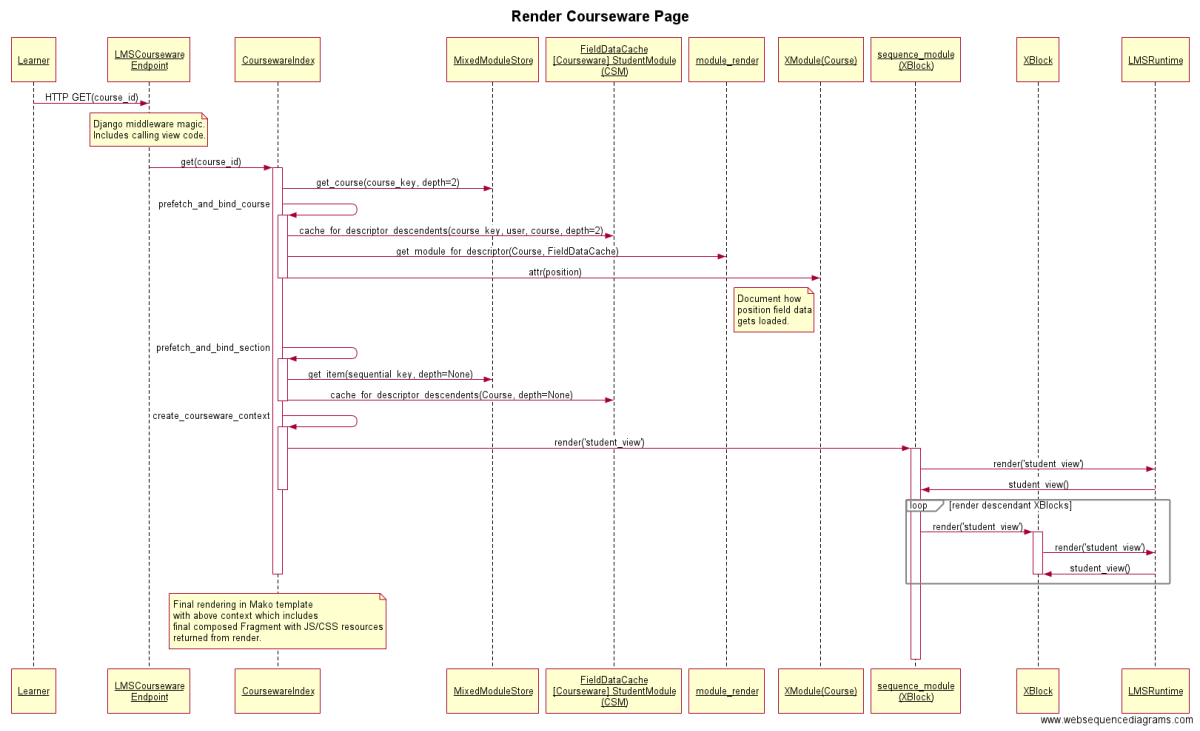
\includegraphics[width=\linewidth]{images/Render_Courseware_Page_Sequence_Diagram.png}
	\caption{Rendering of courseware using XBlocks}
	\label{Fig.1:Sequence diagram}
\end{figure}


\section{Testing and Installing Created XBlock}
\subsection{For Workbench}
We can test a xblock, while running with edX or workbench. Install the xblock using following
commands and start as a local server, and open the browser to find the link for new xblock
\begin{enumerate}
\item Go to the root directory of new created xblock.
\item Type in the following commands\begin{center}\verb= pip install -e name of xblock=\end{center}
\item run the workbench as a local server using command python manage.py
runserver
\end{enumerate}


\subsection{For Open edX instance}
Clone the repository on our local machine. Testing this first on devstack is always recommended
\begin{enumerate}
\item Enter the shell of your devstack and execute :
\begin{center}\verb= sudo -u edxapp /edx/bin/pip.edxapp install /path/to/cloned/directory=\end{center}
\textbf{Note:} You need to point pip to the directory containing setup.py of our project.\newline For
example: If we cloned this repo in directory called\textbf{ /home/edx/advhtmlxblock} and
\textbf{/home/edx/advhtmlxblock/setup.py}is present then\textbf{ /home/edx/advhtmlxblock} is your
required path
\item (Re)start your LMS and CMS.
\item Login to studio as staff
\item Go to "Advanced Settings" in your course
\item Add word advancedhtml to list of "Advanced Modules"
\item Save changes
\item Advanced HTML component should be present in "Advanced" section in your course.
\end{enumerate}


%%%%%%%%%%%%%%%%%%%%%%%%%%%%%%%%%%%%

